\chapter{Graph processing}
\label{chp:graph}

In order to process large graphs, a graph processing system is required.
A graph processing system uses a data model of vertices which are connected by edges~\cite{sakr2013processing}.
Vertices can have an ID and a value, edges can have a direction and a value.
The vertex values are modified during computation, and edges can be added and/or removed during computation.
A graph system can scale out horizontally (linearly with size), and is therefore able to process graph data at large scale.
A large graph system must also be able to handle failover, such as network, storage or hardware failure.
There are multiple graph systems available,
 for example GraphLab~\cite{low2010graphlab}, 
 GraphX~\cite{xin2013graphx}, 
 Pregel~\cite{Malewicz:2010:PSL:1807167.1807184} 
 and Giraph~\cite{avery2011giraph,ching2013scaling}.
This thesis will focus on Giraph,
 but other systems are expected to give similar results.

\section{Bulk Synchronous Parallel model}
\label{sec:bsp}

\begin{figure}[h]
	\caption{BSP programming model~\cite{sakr2013processing}}
	\label{fig:BSP}
	\centering
		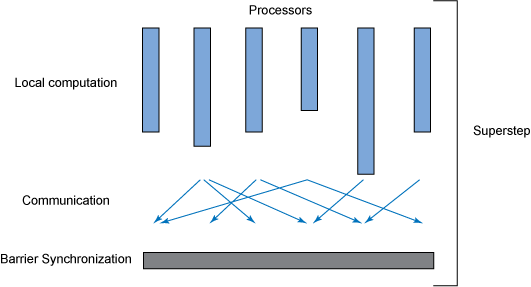
\includegraphics[width=1\textwidth]{BSP}
\end{figure}

By running calculations in parallel, more computations per second are possible.
The case for parallel computing is strengthened by the fact that processing power is cheap nowadays,
 but fast processing is achieved by using many processors in parallel.
Parallel computing does, however, pose an important challenge,
 in that a single processor cannot share memory with another processor, and synchronisation is expensive,
 as it requires processors to wait, as memory cannot be reliably changed by two different processes.

The Bulk Synchronous Parallel model~\cite{Valiant:1990:BMP:79173.79181} (figure~\ref{fig:BSP}) is a model for parallel computing.
It consists of components that handle processing and/or memory.
Operations are divided in so-called supersteps.
A router allows components to exchange point to point messages at the end of a superstep execution,
 which allows for storage access between components.
The model is useful for running large calculations that will take a very long time with standard hardware.

\section{Giraph}
Giraph is a software based implementation of the the Bulk Synchronous Parallel model,
 and allows for a large amount of physical machines to form a cluster.
A Giraph computation program consists of a single \verb"calculate" function, which has two arguments; (1) the vertex and (2) the messages that were sent to the vertex during the last superstep.
During every superstep of the computation, a vertex may send a message to another vertex via one of its outgoing edges.
A vertex may also ``vote to halt'', to indicate that it is done calculating.
If a vertex votes to halt, it will not be called during subsequent supersteps, unless it receives a message from another vertex.
A vertex that has received a message will always be called, and any previous votes to halt are forgotten; the vertex will have to vote to halt again.

Before the computation is started, the graph is read by a \verb"VertexInputFormat" or an \verb"EdgeInputFormat".
After computation, the graph is written by a \verb"VertexOutputFormat" or \verb"EdgeOutputFormat"\footnote{\url{https://giraph.apache.org/io.html}}.
When the program is started, Giraph will start worker processes on the physical machines.
The workers will each read a part of the graph, Giraph will distribute the graph, workers will execute supersteps and after the last step is completed, the workers write their part of the graph.

Giraph takes care of the communication between the workers, and distributes the workload over the workers.
Due to the nature of BSP, it is important for Giraph that every worker will take roughly the same amount of time to complete a superstep.
After each superstep, the nodes have to synchronise and start working on the next superstep, which means that if one worker is slow, all other workers have to wait for it to finish.

\section{Design choices}
\subsection{Optimisations}
When implementing a computation for a graph system, such as Giraph, it is important to make the run-time of each computation as short as possible.
During each superstep, all workers will run computations, so that each vertex is computed once per superstep.
During a single computation, all incoming messages to the vertex for that superstep must be handled, and possibly all outgoing edges must be iterated over to send messages to neighbouring vertices.
Iteration is a weak spot for parallel systems, as it is not executed in parallel.
Therefore, in order to cut on computation time, vertices should have as few edges as possible.
%Section~\ref{sec:model_optimisation} describes how SpreadRank optimises the model.




% "*** Explain a bit how you have done and which choices you made in your thesis work."

